\documentclass[12pt, oneside]{article}   	% use "amsart" instead of "article" for AMSLaTeX format
\usepackage{color}
\usepackage{geometry}                		% See geometry.pdf to learn the layout options. There are lots.
\geometry{letterpaper}                   		% ... or a4paper or a5paper or ... 
%\geometry{landscape}                		% Activate for for rotated page geometry
%\usepackage[parfill]{parskip}    		% Activate to begin paragraphs with an empty line rather than an indent
\usepackage{graphicx}				% Use pdf, png, jpg, or eps§ with pdflatex; use eps in DVI mode
								% TeX will automatically convert eps --> pdf in pdflatex		
\usepackage{amssymb}
\usepackage{amsmath}
\usepackage[compact]{titlesec}
\usepackage{float}
\usepackage{pdflscape}
%\usepackage{rotating}
\usepackage{soul}
%\usepackage{longtable}
%\usepackage{threeparttable}
%\usepackage{lineno}
\usepackage[round]{natbib} %round makes parentheses instead of square brackets
\usepackage{url}
%\usepackage{authblk}
\setcounter{secnumdepth}{4}
\titleformat{\paragraph}
{\normalfont\normalsize\bfseries}{\theparagraph}{1em}{}
\titlespacing*{\paragraph}
{0pt}{3.25ex plus 1ex minus .2ex}{1.5ex plus .2ex}
\graphicspath{ {images/} }

\title{Persistence metrics and data connections}

\begin{document}
%\linenumbers
\date{}
\maketitle{}
\section{Terms}
\begin{itemize}
	\item recruit: fish in the 3.5-6.0cm size class (able to be fin-clipped but not tagged), which preliminary growth analyses suggest settled the previous year and are about one year old (will refine growth analyses to confirm/check)
	\item LEP (lifetime egg production): the expected reproductive output in terms of eggs of one individual, considering only reproduction as a female
	\item LR (local retention): recruits returning home over total output of recruits from the patch
		\begin{equation}
			\begin{split}
				LR & = \frac{\text{\# arrivals returning home}}{\text{output from patch}} \\
				   & = \frac{\text{\# recruits arriving home}}{\text{ \# recruits produced by patch}} \\
				   & = \frac{p_{i,i} \times \text{\# recruits from site}}{\frac{\text{recruits}}{\text{egg}} \times \text{\# eggs produced by site}}
			\end{split}
		\end{equation}
	\item $p_{i,j}$: of recruits from patch $i$ that recruited somewhere, the probability of dispersing from patch i to patch j
	\item $p_{\text{hab}}$: proportion of habitat sampled (estimated as number of anemones visited over estimated total number of anemones at site)
	\item $p_{\text{cap}}$: probability of sampling a fish, given that we visited its anemone (estimated using mark-recapture within a sampling season)
\end{itemize}

\section{Network persistence: demographic connectivity matrix}
A group of patches are network persistent if the largest eigenvalue of the demographic connectivity matrix (C) is $ > 1$ (\cite{burgess2014beyond,lyselpopulation})
\begin{equation}
C_{ij} = LEP_i \times \frac{\text{recruits}}{\text{egg}} \times p_{ij}.
\end{equation}

Calculate this metric for both the overall population and smaller groups of patches within the network, to see at what scale persistence might occur.

% \begin{equation}
% \text{realized connectivity matrix} = \text{reproductive output (in terms of "recruits")} \times \text{dispersal prob (for "recruits")} \times \text{probability of survival to maturity for females}
% \end{equation}

\section{Self-persistence}
A patch is self-persistent (\cite{burgess2014beyond}) if
\begin{equation}
LEP \times LR \geq 1,
\end{equation}
where both LEP and LR consider the same life stage, essentially seeing whether an individual will be able to replace itself, considering its total lifetime reproductive output, the survival of that output to recruitment, and the probability that recruitment returns to the natal patch.

So, for recruits as the starting age and fecundity and LEP in terms of eggs, you get:
\begin{equation}
SP_i = LEP_{i} \times \frac{\text{recruits}}{\text{egg}} \times \frac{p_{i,i} \times \text{\# recruits from site}}{\frac{\text{recruits}}{\text{egg}} \times \# \text{eggs produced by patch i}} \geq 1, 
\end{equation}

which simplifies to
\begin{equation}
SP_i = LEP_{i} \times \frac{\text{recuits}}{\text{egg}} \times p_{i,i} \geq 1 \label{SP_simp_v2}, %IS THIS RIGHT? CHECK / THINK THROUGH THIS AGAIN... SHOULD CHAT WITH MP AND KC ABOUT THIS, RUN BY MICHAEL BODE ONCE HAVE OTHER METRICS IN PLACE
\end{equation}
(and is the diagonal entries of $C$). \\

Or, alternately, could write it as:
\begin{equation}
SP_i = LEP_{i} \times \frac{\text{recruits}}{\text{egg}} \times \frac{\# \text{recuits arriving home to patch i}}{\frac{\text{recruits}}{\text{egg}} \times \# \text{eggs produced by patch i}} \geq 1, 
\end{equation}

which simplifies to be

\begin{equation}
SP_i = LEP_{i} \times \frac{\# \text{recuits arriving home to patch i}}{\# \text{eggs produced by patch i}} \geq 1 \label{SP_simp_v1}. %IS THIS RIGHT? CHECK / THINK THROUGH THIS AGAIN... SHOULD CHAT WITH MP AND KC ABOUT THIS, RUN BY MICHAEL BODE ONCE HAVE OTHER METRICS IN PLACE
\end{equation}
% where

% \begin{itemize}
	
	
% \end{itemize}

% % where here LEP (lifetime egg production) is the reproductive output in terms of recruits from recruitment to death. Here, will define recruit for both the starting point of the LEP calculation and the stage of offpsring assessed as fish in the 3.5-6.0cm size range, which preliminary growth analyses suggest are fish that are about one year old and settled the previous year. Here, we will assess the starting age for LEP and  both the recruit stage and the offspring produced to be fish that are one year old, so spawned and settled the previous year, which we are assuming are fish in the 3.5-6.0cm size range based on preliminary growth analyses (though need to confirm with updated growth curve). To assess whether replacement is achieved, we will asu


% LEP is calculated by:

% \begin{equation}
% LEP = \Sigma_{a = 1}^{A} l(a)f(a),
% \end{equation}{}'

% where $a$ is age, starting at age of recruitment, $A$ is age of death, $f(a)$ is fecundity at age $a$, and $l(a)$ is survival from recruitment to age $a$. Fecundity could be considered in terms of eggs or could include some mortality and be defined in terms of larvae, juveniles, recruits, etc. LEP could have site-specific survivals and fecundities.\\ %Is this right for l(a)??? 

% LR (local retention) is the fraction of larvae (or other stage) that are produced by a patch that return to settle,

% \begin{equation}
% \begin{split}
% LR & = \frac{\text{\# arrivals returning home}}{\text{output from patch}} \\
% & = \frac{\text{\# recruits arriving home}}{\text{ \# recruits produced by patch}} \\
% & = \frac{p_{\text{dispersing home}} \times \text{\# recruits from site}}{\frac{\text{recruits}}{\text{eggs}} \times \text{\# eggs produced by site}}
% \end{split}
% \end{equation}

% For this to work, the life stage considered as offspring in LEP and the life stage in LR should be the same. Basically, this is seeing whether a reproductive individual will be able to replace itself, considering its total lifetime output (and the survival of that output to a recruitment stage) and the probability of that output returning to its natal patch. Breeding females or 3.5cm 

% Putting this all together, for a 3.5cm recruit as the starting age and fecundity in terms of eggs, you get:
% \begin{equation}
% SP_i = LEP_{i, \text{$a_0$ = 3.5cm}} \times \frac{\text{recruits}}{\text{egg}} \times \frac{\text{recuits arriving home to patch i}}{\frac{\text{recruits}}{\text{egg}} \times \# \text{eggs produced by patch i}} \geq 1, 
% \end{equation}

% which simplifies to be

% \begin{equation}
% SP_i = LEP_{i, \text{$a_0$ = 3.5cm}} \times \frac{\text{recuits arriving home to patch i}}{\# \text{eggs produced by patch i}} \geq 1. %IS THIS RIGHT? CHECK / THINK THROUGH THIS AGAIN... SHOULD CHAT WITH MP AND KC ABOUT THIS, RUN BY MICHAEL BODE ONCE HAVE OTHER METRICS IN PLACE
% \end{equation}

% Or, could be
% \begin{multline}
% SP_i = LEP_{i, \text{$a_0$ = 3.5cm}} \times \frac{\text{recruits}}{\text{egg}} \times \\ \frac{p_{\text{dispersing home}} \times \text{\# recruits from site}}{\frac{\text{recruits}}{\text{egg}} \times \# \text{eggs produced by patch i}} \geq 1, 
% \end{multline}

% which simplifies to
% \begin{equation}
% SP_i = LEP_{i, \text{$a_0$ = 3.5cm}} \times \frac{\text{recuits}}{\text{eggs}} \times p_{\text{dispersing home}} \geq 1. %IS THIS RIGHT? CHECK / THINK THROUGH THIS AGAIN... SHOULD CHAT WITH MP AND KC ABOUT THIS, RUN BY MICHAEL BODE ONCE HAVE OTHER METRICS IN PLACE
% \end{equation}

\section{Connections with data}
\begin{itemize}
	\item LEP: use survival-by-size estimates from mark-recapture, growth estimates from mark-recapture, fecundity estimates from egg photos (preliminary numbers and relationship with size in progress by Adam) to estimate LEP with an integral projection model
	\item output in eggs from each site:
	$N_{\text{eggs}, i} = \# \text{females} \times p_{\text{hab}} \times p_{\text{cap}} \times \text{fecundity}$, with fecundity estimates from photos (might be related to size, depending on relationship) and clutches-per-year data from \cite{holtswarth2017fecundity}.
	\item $p_{i,j}$, version 1: integrate the dispersal kernel estimated with the \cite{bode2018estimating} method (kernel-fitting being done by Katrina using parentage data and proportion habitat sampled) over the distances between sites
		\begin{itemize}
			\item kernel is a Laplacian kernel with parameters $k$ (scale parameter) and $\theta$ (exponent) and depends on distance $x$: $f(x,k,\theta)$
			\item after normalization, the kernel gives the probability of recruiting distance $x$ away from origin, given that you recruited somewhere
			\item $d1$: distance between the mid-point of site $i$ and the closest edge of site $j$ 
			\item $d2$: distance between the mid-point of site $i$ and the farthest edge of site $j$
			\item integrate to get probability of recruiting at site $j$ from site $i$, given that you recruited somewhere
			\begin{equation}
			p_{i,j} = \int_{d1}^{d2}{f(x,k,\theta) dx}. \label{PijfromKernel}
			\end{equation}
		\end{itemize}
	\item $p_{i,j}$, version 2: estimate from the proportion-of-recruitment connectivity matrix generated by the \cite{wang2014estimation} (MigEst) method (migration estimates being done by Katrina using the parentage and data and proportion habitat sampled) 
		\begin{itemize}
			\item the output of MigEst is an $s$ (destination) by $t$ (source) matrix $M$, where $s$ is the number of sampled patches and there is an additional column for unsampled ghost populations ($t = s+1$)
			\item the matrix entries $m_{s,t}$ are the proportion of recruits at site $s$ that come from site $t$ (the row sums - recruits coming to site $s$ - are 1)
			\item $N_{r_s}$: vector of the number of recruits arriving at each site $s$, found by scaling up the number of sampled recruits by the proportion of habitat sampled
			\item $N_{o_t}$ = $N_{\text{eggs produced}_t} \times \frac{\text{recruits}}{\text{egg}}$: vector of number of recruits produced by each source site $t$
			\item convert migration estimates ($m_{s,t}$) from MigEst to proportion of recruits from site $i$ settling at site $j$:
			\begin{equation}
			p_{i,j} = \frac{m_{s,t} \times N_{r_s}}{N_{o_t}}. \label{PijfromMigEst}
			\end{equation}
		\end{itemize}
	% \item $\# \text{eggs produced by } i$ (equals $N_{o_t}$ above): fecundity (either average or size-specific), estimated by Adam egg photo work, multiplied by the estimated number of breeding females at a site (either total or by size), estimated using number of fish caught scaled up by proportion habitat sampled and probability of capturing a fish (estimated by mark-recapture dives within the same year) 
	\item $\frac{\text{recruits}}{\text{eggs}}$: relationship between $\frac{\text{eggs}}{m^2}$ and $\frac{\text{recruits}}{m^2}$ the following year, estimated at a site level and where estimates of both egg production and recruits have been scaled up to account for the proportion of habitat sampled in each year and the probability of sampling a fish given that we covered its anemone (see \ref{FIG_EggRecruitRelbyArea})
	\item $\# \text{recruits arriving home to patch i}$: take raw number of parentage matches matched from site $i$ to $i$ and scale up by proportion habitat sampled (will be an underestimate of self-persistence but could be worth doing as a comparison)

\section*{Plots}
%Egg-recruit relationship
\begin{figure}[H] %Eggs/recruits relationship
    \centering
    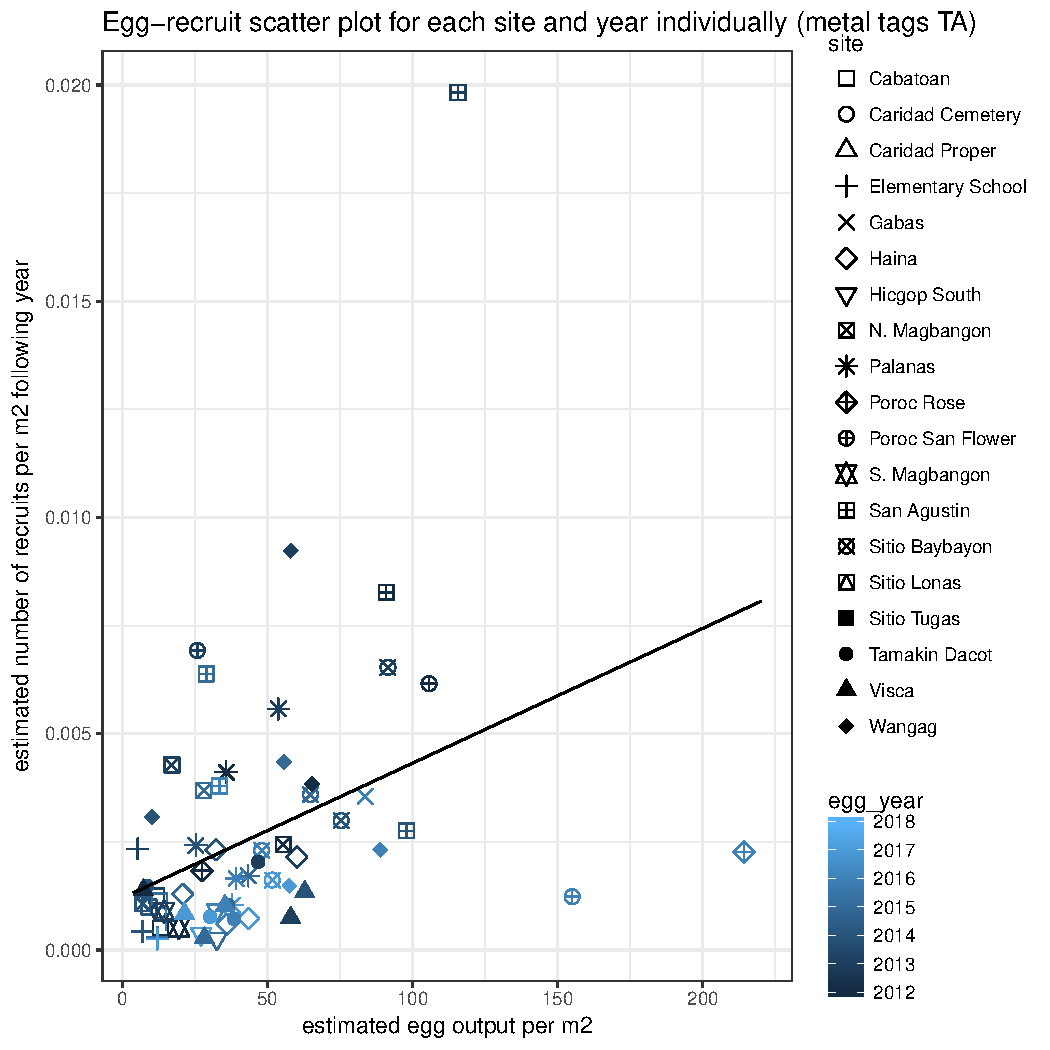
\includegraphics[width=0.8\textwidth]{\detokenize{../Plots/EggRecruitRelationship/Eggs_recruits_by_site_metalTA_m2.pdf}}
    \caption{Plot with best-fit linear line for estimated eggs output (number of females sampled scaled by probability of catching a fish and proportion of habitat sampled and estimated eggs produced per female per year) and the estimated number of recruits (number of recruits sampled scaled by probability of catching a fish and proportion of habitat sampled) in the following year, both scaled by site area. $R^2$ = 0.1509, p-value of F-statistic = 0.00166. \label{FIG_EggRecruitRelbyArea}}
\end{figure}
	
%Estimated growth from mark-recap data
\begin{figure}[H] 
    \centering
    \includegraphics[width=0.8\textwidth]{\detokenize{../../Growth/plots/GrowthPerYear_L1_6mobetween.pdf}}
    \caption{Calculated growth-per-year in cm compared to starting length for fish recaptured at least 6 months after initial capture. Fish caught multiple times are represented as separated catch-recapture pairs, with each recapture compared to the previous capture. Evidence that fish can grow to about 5-6cm within a year? \label{FIG_Growth_L1}}
\end{figure}

%Best-fit VonBL growth curve
\begin{figure}[H] 
    \centering
    \includegraphics[width=0.8\textwidth]{\detokenize{../../Growth/plots/K-S_newData.pdf}}
    \caption{Estimated VonBert growth curve \label{FIG_VonBert}}
\end{figure}

% %Best-fit survival
% \begin{figure}[H] %Eggs/recruits relationship
%     \centering
%     \includegraphics[width=0.8\textwidth]{\detokenize{../../Growth/plots/K-S_newData.pdf}}
%     \caption{Estimated VonBert growth curve \label{FIG_VonBert}}
% \end{figure}

%Network persistence, multiple methods
\begin{figure}[H] 
    \centering
    \includegraphics[width=1.0\textwidth]{\detokenize{../Plots/PersistenceMetrics/NP_realizedconnectivity.pdf}}
    \caption{Network persistence metric (first eigenvalue of realized connectivity matrix), multiple methods. \label{FIG_NP_Metric}}
\end{figure}

%Connectivity matrix eigenvalues, multiple methods
\begin{figure}[H] 
    \centering
    \includegraphics[width=1.0\textwidth]{\detokenize{../Plots/PersistenceMetrics/Eig_connmats.pdf}}
    \caption{First eigenvalue of connectivity matrices, multiple methods. \label{FIG_Conn_Eig}}
\end{figure}

%Self persistence
\begin{figure}[H]
    \centering
    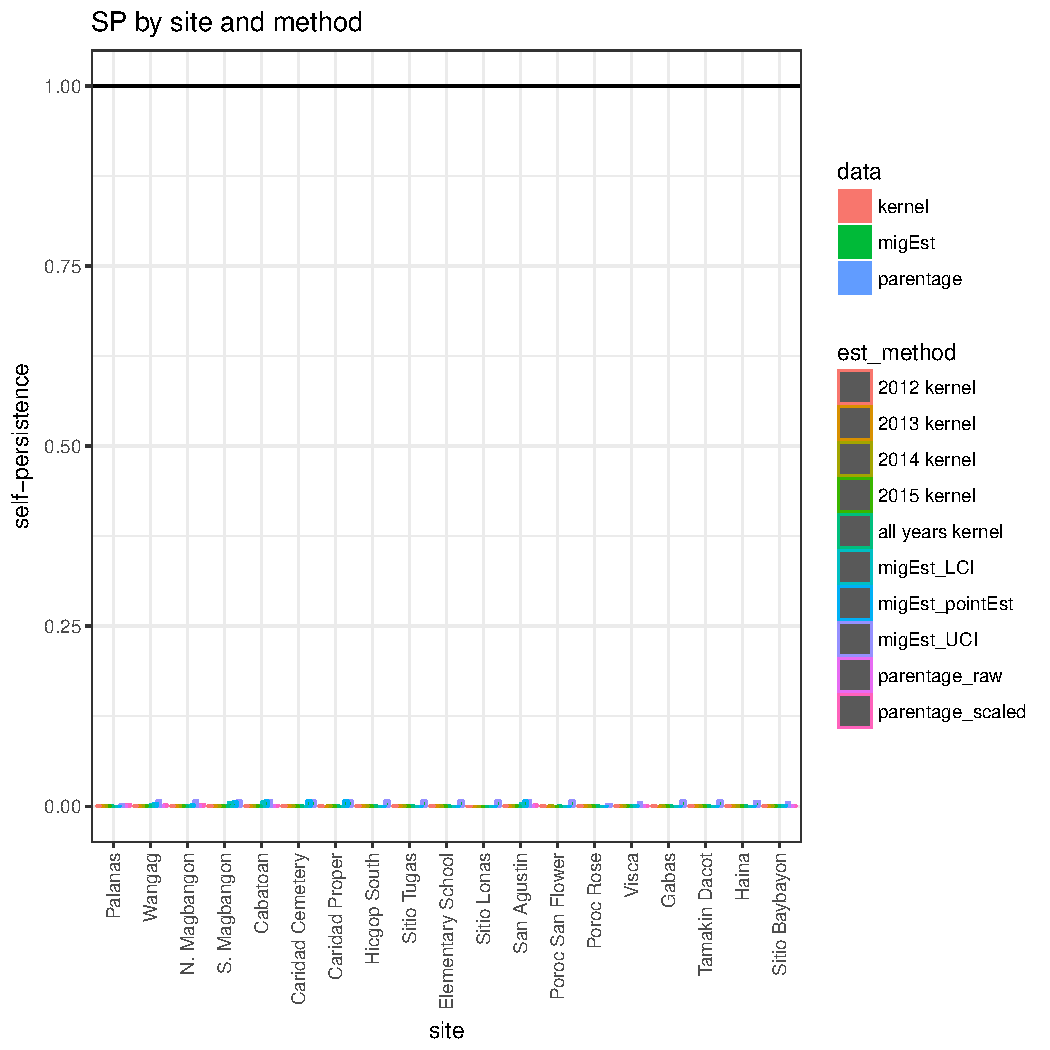
\includegraphics[width=0.8\textwidth]{\detokenize{../Plots/PersistenceMetrics/SP_allmethods.pdf}}
    \caption{Self-persistence, variety of methods. \label{FIG_SP}}
\end{figure}

%Connectivity matrix, all years kernel
\begin{figure}[H] 
    \centering
    \includegraphics[width=1.0\textwidth]{\detokenize{../Plots/PersistenceMetrics/Connectivity_allyears_kernel.pdf}}
    \caption{Connectivity matrix, calculated from all years dispersal kernel. \label{FIG_ConnMat_AllYearsDK}}
\end{figure}

%Connectivity matrix, migEst
\begin{figure}[H] %Eggs/recruits relationship
    \centering
    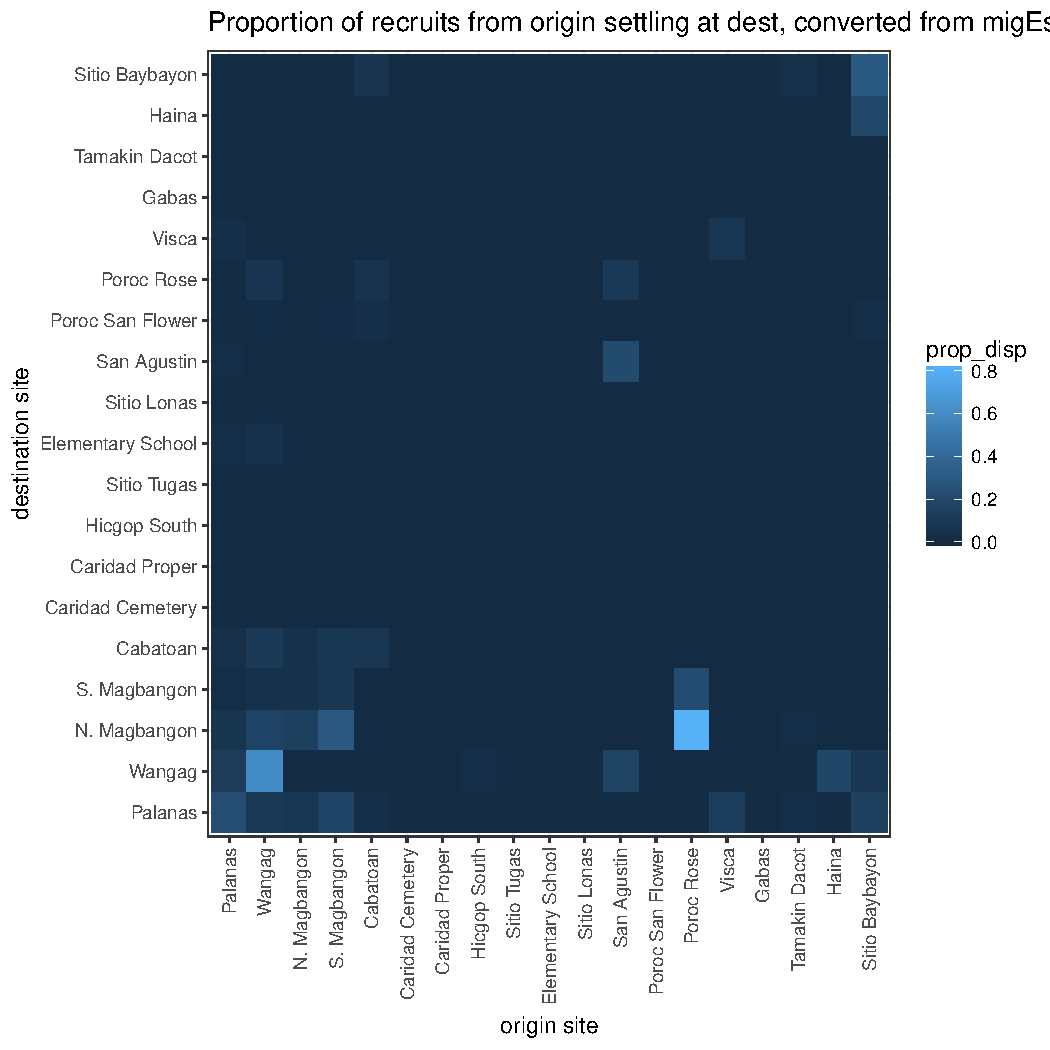
\includegraphics[width=1.0\textwidth]{\detokenize{../Plots/PersistenceMetrics/MigEst_propdisp_mat.pdf}}
    \caption{Connectivity matrix, calculated from migEst values. \label{FIG_ConnMat_AllYearsMigEst}}
\end{figure}

% \item $A$: assuming fish are 1 when they hit 3.5cm, can use the max number of years a fish has been recaught (checking with a histogram that this a minority of fish and likely that we have caught the tail, not the majority) or a number from the literature or annual average survival multipled until proportion surviving is $<$ some threshold (1\%?)
% \item $f(a)$: can start with an average number of eggs per female multiplied by average number of reproductive events per year from Adam's work, then can nuance with size of female (and age from Michelle's growth work or a von-Bertalanffy to estimate age from size), if necessary. Then need to to multiply by probability of surviving from egg to recruit (either here or outside the sum). Or use IPM like Will White did to get at size effects on survival and egg production. %Need to check: can you estimate age from size using a vB? Probably, think Lewis did it in that rockfish paper...
% \item $l(a)$: Use survival-at-size relationship to estimate annual survival at each size (or just use an annual survival) and multiply together to get survival to each age. This is survival from first age of reproduction to the other stages or survival from some other stage to the various ages - need to make sure that is really clearly defined. Could be lifetime egg production of a breeding female, of a 3.5cm recruit, or a larvae, etc.
% \item $\# \text{eggs produced by patch i}$: fecundity (either average or size-specific) multiplied by the estimated number of breeding females at a site (either total or by size)
% \item $\# \text{recruits arriving home to patch i}$: KC's dispersal kernel  (which is prob of dispersing a certain distance, given that you are a settled recruit) multiplied by the number of recruits arriving at that site? \\
% \[
% \text{recruits arriving home} = \text{\# recruits from the site} \times p_{\text{dispersing w/in site}}
% \],
% where $p_{\text{dispersing w/in site}}$ is the dispersal kernel integrated over the site width and represents the probability of settling within site boundaries, given that you settled somewhere, and $\text{\# recruits from the site}$ is the number of recruits that settled somewhere produced from site $i$. This can be calculated as 
% \item Can estimate egg-recruit survival ($\frac{\text{recruits}}{\text{egg}}$) by getting the number of 3.5cm-sized fish (or recruit defined at a different stage - reproductive fish, reproductive female) at each patch compared to the number of eggs produced by the patch the year before. This assumes eggs only recruit to their patch, though, which is what we're trying to test here, so would want to consider these ratios at different spatial scales, like the whole population together. Need to think about this a bit more. Given the number of females out there in each patch and overall population, how many recruits do we see the next year?
% \item 
% \item $\# \text{recruits arriving home to patch i}$ (alternate): could just use raw \# of parentage matches found returning home and scale that by the estimated proportion of the site sampled (only works if we actually get some self-recruits for some of the sites, though - and would be a pretty rough estimate)
\end{itemize}

% \section*{Network persistence: shortfall of SP}
% \subsection*{Metric}
% A patch is persistent through network persistence if it is persistent but not through self-persistence.

% \begin{equation}
% P_i = LEP_{i, \text{$a_0$ = 3.5cm}} \times \frac{\# \text{recuits arriving to patch i}}{\# \text{eggs produced by patch i}} \geq 1. %IS THIS RIGHT? CHECK / THINK THROUGH THIS AGAIN... SHOULD CHAT WITH MP AND KC ABOUT THIS, RUN BY MICHAEL BODE ONCE HAVE OTHER METRICS IN PLACE
% \end{equation}

% Assess persistence by:
% \begin{equation}
% \frac{\text{recruits}}{\text{female}}*\text{survival to breeding} \geq \text{annual mortality}*N_{\text{females}}
% \end{equation}

% Or, could assess persistence in the same way as self-persistence but use all recruits coming to the site as the numerator. If it is persistent but not self-persistent, must be through network persistence (so if $P_i \geq 1$ but $SP_i < 1$).

% \subsection*{Data}
% \begin{itemize}
% 	\item $\frac{\text{recruits}}{\text{female}}$: LEP from stage of breeding female (rather than 3.5cm as above) multiplied by survival of eggs to recruits (either estimated from relationship or from literature)
% 	\item survival to breeding: use annual survival to estimate survival from recruitment (3.5 or whatever) to breeding female
% 	\item annual mortality for breeding females: same as used in LEP above, have from mark-recap
% 	\item $N_{\text{females}}$: estimated at a site by scaling up $N_{\text{captured}}$ by prob of catching a female (could redo Lincoln-Peterson for just breeding females) and proportion of site sampled
% 	\end{itemize}

% \section*{Network persistence: demographic connectivity matrix}
% A group of patches are network persistent if the largest eigenvalue of the demographic connectivity matrix (C) is $ > 1$ (\cite{burgess2014beyond,lyselpopulation})
% \begin{equation}
% C_{ij} = LEP_i \times p_{ij},
% \end{equation}

% where $LEP_i$ is the lifetime egg production at patch i and $p_{ij}$ is the probability of a recruit dispersing from patch i to patch j.

% \begin{equation}
% \text{realized connectivity matrix} = \text{reproductive output (in terms of "recruits")} \times \text{dispersal prob (for "recruits")} \times \text{probability of survival to maturity for females}
% \end{equation}

% \section*{Equations for presentation}
% Just means they are clean and don't have extraneous punctuation or unexplained indexing and such...
% \begin{equation}
% SP = LEP \times LR \geq 1
% \end{equation}

% \begin{equation}
% LEP = \Sigma_a^A l(a)f(a)
% \end{equation}

% \begin{equation}
% LR = \frac{\text{\# arrivals returning home}}{\text{output from patch}}
% \end{equation}

% \begin{equation}
% SP_i = LEP_{i} \times \frac{\text{recuits arriving home to patch i}}{\# \text{eggs produced by patch i}} \geq 1 %IS THIS RIGHT? CHECK / THINK THROUGH THIS AGAIN... SHOULD CHAT WITH MP AND KC ABOUT THIS, RUN BY MICHAEL BODE ONCE HAVE OTHER METRICS IN PLACE
% \end{equation}

% \begin{equation}
% NP_i = LEP_{i} \times \frac{\text{recuits arriving to patch i}}{\# \text{eggs produced by patch i}} \geq 1 %IS THIS RIGHT? CHECK / THINK THROUGH THIS AGAIN... SHOULD CHAT WITH MP AND KC ABOUT THIS, RUN BY MICHAEL BODE ONCE HAVE OTHER METRICS IN PLACE
% \end{equation}

% \begin{equation}
% C_{ij} = LEP_i \times p_{ij}
% \end{equation}

%\section*{Input-output balance}

%\section*{Recuits/female}

% \section*{Looking at the literature}
% What have other papers done? How/where have they accounted for larval mortality (or pre-recruitment mortality)? What is their dispersal kernel conditional on? What does it sum to?
% \subsection*{Papers to look at}
% \begin{itemize}
% 	\item \cite{johnson2018integrating}
% 	\item \cite{carson_reproductive_2010}
% 	\item \cite{salles2016genetic}
% \end{itemize}
% \subsection*{Summaries of what others have done}

\newpage{}

\bibliography{../../../BibTexReferences}
\bibliographystyle{plainnat}

\end{document}